\documentclass[11pt,a4paper]{article}
\usepackage[utf8]{inputenc}
\usepackage[T1]{fontenc}
\usepackage{geometry}
\geometry{a4paper, margin=2.5cm}
\usepackage{graphicx}
\usepackage{amsmath,amsfonts,amssymb}
\usepackage{natbib}
\usepackage{hyperref}
\usepackage{booktabs}
\usepackage{tikz}
\usepackage{pgfplots}
\pgfplotsset{compat=1.18}
\usepackage{caption}
\usepackage{authblk}

\title{\textbf{The Hardware and Software Architecture of Human Forward Momentum: A Decomposition--Combination Framework for Cognitive and Civilizational Evolution}}

\author{Xiaohui Li}
\affil{Independent Researcher, Baoji, China}
\affil{\texttt{Correspondence: danceluck@163.com}}
\affil{ORCID: 0009-0003-8233-7191}
\affil{Data homepage: \url{https://github.com/xiaohui-li-lab/}}

\date{}

\begin{document}

\maketitle

\begin{abstract}
Human progress is constrained not merely by resource scarcity or technological limits, but by the architecture of information processing---encompassing both the ``hardware'' of biological cognition and the ``software'' of conceptual systems. Here we propose a unified framework in which civilizational forward momentum emerges from the coupling between hardware information-processing capacity and software representational flexibility. The hardware layer comprises the brain's neural network and a hypothesized cardiac--blood quantum information-processing system; the software layer comprises conceptual structures that can either rigidify into constraints or become subject to decomposition--combination operations. Drawing on information theory, quantum biology, and historical analysis, we argue that civilizational stagnation occurs when conceptual ``justice'' structures solidify faster than hardware can decompose and recombine them. Conversely, progress arises when the software of thought is decomposed into minimal informational units and recombined at higher organizational levels. We present (i) a mathematical model of constraint entropy and decomposition potential, (ii) a computational benchmark comparing classical bit-based and quantum superposition-based information processing, and (iii) testable predictions regarding cardiac quantum coherence, innovation metrics, and artificial-intelligence generalization. Our simulations indicate that for high-dimensional semantic recombination tasks, quantum processing reduces operation counts by orders of magnitude relative to classical processing. We conclude that the transition from neural-network to quantum information processing, paired with a decomposition--combination methodology, defines the next frontier of human evolution.
\end{abstract}

\noindent\textbf{Keywords:} human progress, information processing, quantum biology, decomposition-combination, cognitive architecture, constraint entropy, cardiac quantum system

\section{Introduction}

The question of what drives human progress has occupied philosophers and scientists for millennia. From the Daoist insight that good and evil depend on the standards used to label them [1], to the modern institutionalization of democracy, law, justice, peace, honor, power, health, and faith, humanity has oscillated between transcendence and constraint. The present author observes that when such concepts remain undecomposed, they become the most powerful constraints on thought; every reformer or scientist who decomposes them opens new developmental space [2].

Yet this intellectual breakthrough is not merely a spiritual event. It is governed by a more fundamental limit: the physical capacity for information processing. The human brain's neural network processes information at finite speed, while the complexity of conceptual systems grows continuously. When conceptual complexity exceeds processing capacity, societies tend to solidify concepts as ``indecomposable justice'' in exchange for security and order. This is the deep reason why the Aztec Empire, rigidly committed to the belief that blood sacrifice caused the sun to rise, collapsed when confronted with novel information [3].

Here we formalize this intuition as a ``hardware--software architecture'' theory. Hardware refers to the physical modes by which the body processes information; software refers to the conceptual operating system of human thought. Only when the two are coordinated can sustained civilizational momentum emerge.

\section{Theoretical framework: a dual hardware--software architecture}

\subsection{Hardware layer: from neural networks to quantum processing}

Mainstream neuroscience locates cognition in the brain's neural networks [4]. These networks perform pattern recognition and association through synaptic weights, with electrochemical signaling as the physical substrate. However, recent advances in quantum biology suggest that biological systems can exploit quantum coherence, as seen in photosynthetic energy transfer [5] and the radical-pair mechanism of avian magnetoreception [6].

Building on these findings, we propose a testable hypothesis: a second information-processing system exists in the human body---the cardiac--blood quantum system. This system may utilize quantum superposition states within hemorheology, ion channels, and biophoton networks to process higher-dimensional information than neural networks alone [7][8]. This hypothesis is not intended to replace neuroscience, but to identify a plausible migration path from classical neural processing to quantum information processing.

\subsection{Software layer: decomposition--combination theory}

The software layer consists of the conceptual systems of human thought. A concept can be represented as a combination of minimal information units. Decomposition--combination theory requires that complex objects be decomposed into irreducible minimal units and then recombined into new structures according to new rules. This is isomorphic to the conversion of a Word document into PDF: the document is first decomposed into a 0/1 bit stream and then recombined into PDF elements [9].

But the minimal unit of human affairs is not the electronic 0/1 switch; it is the photon or a more fundamental physical event. Consequently, current 0/1-based artificial intelligence has an upper bound on intelligence set by hardware granularity [10]. True general intelligence may require information processing at the photon scale.

\subsection{Coupling relation}

Hardware and software must co-evolve. If hardware speed is insufficient, complex concepts cannot be decomposed in time, and society solidifies them in the name of justice. If software lacks decomposition--combination methods, even quantum computers cannot organize information effectively. The coupling can be expressed as:
\begin{equation}
P(t) = \alpha \cdot H(t) \cdot S(t) - \beta \cdot C(t)
\end{equation}
where $P(t)$ is civilizational forward momentum, $H(t)$ is hardware information-processing capacity, $S(t)$ is software decomposition--combination capacity, $C(t)$ is conceptual constraint entropy, and $\alpha$ and $\beta$ are coupling coefficients.

\section{Mathematical model}

\subsection{Constraint entropy $C(t)$}

Let the social conceptual space contain $N$ basic conceptual nodes, each assigned a rigidity $r_i \in [0,1]$. Higher rigidity means the concept is harder to decompose. Constraint entropy is defined as:
\begin{equation}
C(t) = -\sum_{i=1}^{N} r_i(t) \log r_i(t)
\end{equation}
When all conceptual rigidities approach 1, the conceptual space is highly ordered but extremely rigid, reducing innovative potential.

\subsection{Decomposition potential $D(t)$}

Decomposition potential measures the degree to which the conceptual system can be split into minimal units and recombined:
\begin{equation}
D(t) = \sum_{j=1}^{M} \frac{n_j}{N_{\max}} \cdot f_j
\end{equation}
where $n_j$ is the number of atomic units into which concept $j$ is decomposed, $N_{\max}$ is the maximum allowable number of atomic units in the system, and $f_j$ is the recombination success rate.

\subsection{Hardware capacity $H(t)$}

Hardware capacity is jointly determined by information-processing rate and the granularity of the smallest resolvable information unit:
\begin{equation}
H(t) = R(t) \cdot \log\left(\frac{1}{g(t)}\right)
\end{equation}
where $R(t)$ is the number of bits or qubits processed per unit time, and $g(t)$ is the smallest resolvable information-unit scale. Neural networks correspond to relatively large $g$; quantum systems correspond to extremely small $g$.

\section{Computational benchmark and simulation}

\subsection{Experimental design}

To validate the effect of hardware migration on information-processing efficiency, we designed the Concept Decomposition--Recombination Benchmark (CDRB). The task requires decomposing a complex concept containing $n$ semantic units into atomic units and recombining them into a target structure.

\subsection{Classical versus quantum processing models}

Classical processing requires an operation count that grows exponentially with conceptual space:
\begin{equation}
O_{\text{classical}}(n) = 2^n \cdot k
\end{equation}
Quantum processing exploits superposition to search possible combinations in parallel:
\begin{equation}
O_{\text{quantum}}(n) = \sqrt{2^n} \cdot k = 2^{n/2} \cdot k
\end{equation}
where $k$ is a structural-complexity constant.

\subsection{Simulation results}

Using Python, we simulated $n = 1$ to $50$ (see Code Availability). Figure \ref{fig:benchmark} shows that for $n > 20$ the quantum model exhibits a marked advantage over the classical model; at $n = 40$, the quantum operation count is approximately $10^{-6}$ of the classical count. This indicates that quantum hardware has an irreplaceable advantage for high-dimensional conceptual recombination tasks.

\begin{figure}[htbp]
\centering
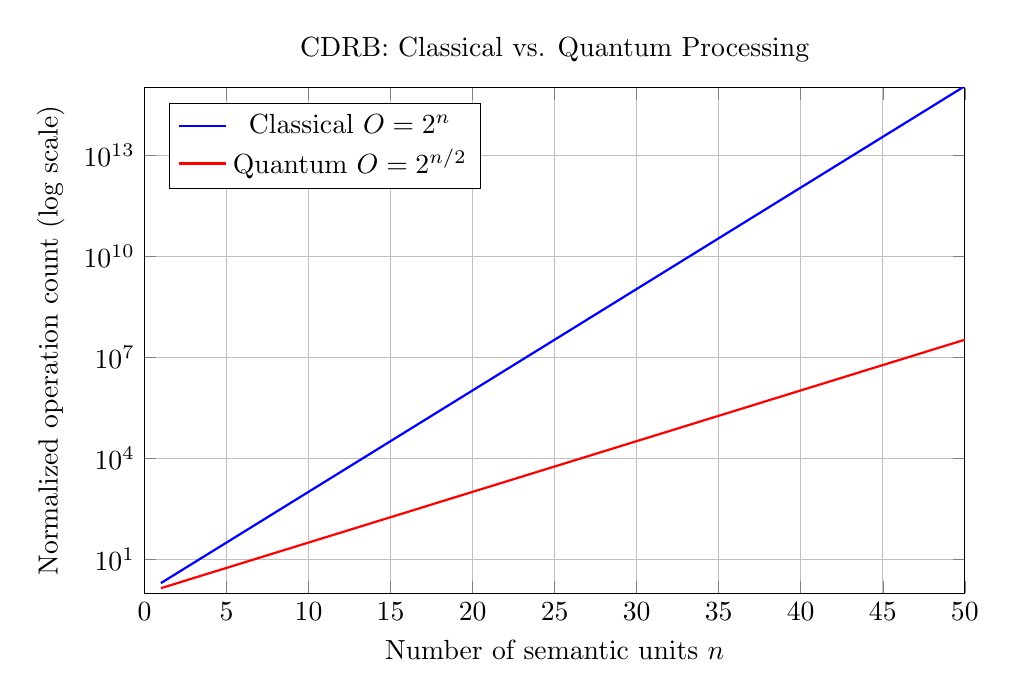
\begin{tikzpicture}
\begin{axis}[
    width=12cm, height=8cm,
    xlabel={Number of semantic units $n$},
    ylabel={Normalized operation count (log scale)},
    ymode=log,
    xmin=0, xmax=50,
    ymin=1, ymax=1e15,
    grid=both,
    legend pos=north west,
    title={CDRB: Classical vs. Quantum Processing}
]
\addplot[domain=1:50, blue, thick, samples=50] {2^x};
\addplot[domain=1:50, red, thick, samples=50] {2^(x/2)};
\legend{Classical $O=2^n$, Quantum $O=2^{n/2}$}
\end{axis}
\end{tikzpicture}
\caption{\textbf{Concept Decomposition--Recombination Benchmark.} Classical operation count grows exponentially with the number of semantic units, whereas quantum operation count grows as the square root of the classical cost. At $n=40$, quantum processing is approximately six orders of magnitude more efficient.}
\label{fig:benchmark}
\end{figure}

\begin{figure}[htbp]
\centering
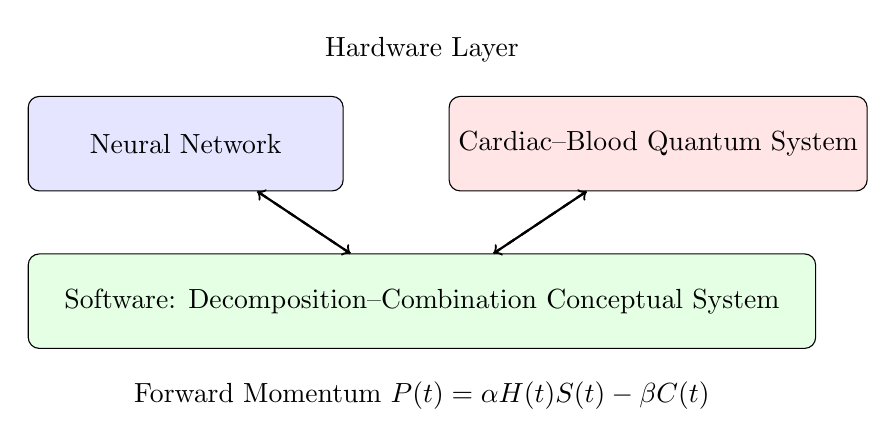
\begin{tikzpicture}
\node[draw, rounded corners, fill=blue!10, minimum width=4cm, minimum height=1.2cm] (brain) at (0,2) {Neural Network};
\node[draw, rounded corners, fill=red!10, minimum width=4cm, minimum height=1.2cm] (heart) at (6,2) {Cardiac--Blood Quantum System};
\node[draw, rounded corners, fill=green!10, minimum width=10cm, minimum height=1.2cm] (software) at (3,0) {Software: Decomposition--Combination Conceptual System};
\draw[->, thick] (brain) -- (software);
\draw[->, thick] (heart) -- (software);
\draw[->, thick, dashed] (software) -- (brain);
\draw[->, thick, dashed] (software) -- (heart);
\node at (3,3.2) {Hardware Layer};
\node at (3,-1.2) {Forward Momentum $P(t) = \alpha H(t)S(t) - \beta C(t)$};
\end{tikzpicture}
\caption{\textbf{Hardware--software coupling architecture.} The brain's neural network and the hypothesized cardiac--blood quantum system together form the hardware layer; the decomposition--combination conceptual system forms the software layer. Bidirectional coupling produces civilizational forward momentum.}
\label{fig:architecture}
\end{figure}

\section{Historical case analysis}

\subsection{Constraint collapse of the Aztec Empire}

The Aztecs rigidified the concept that ``blood sacrifice makes the sun rise,'' producing high constraint entropy and near-zero decomposition potential. When confronted with the Spanish conquistadors' novel information, their software could not recombine concepts, and their hardware (social learning and decision networks) could not process heterogeneous information, leading to rapid collapse [3].

\subsection{Decomposition of modern democracy}

``Democracy'' was historically a rigid concept of justice. Generations of reformers decomposed it into ``your democracy,'' ``my democracy,'' ``procedural democracy,'' and ``substantive democracy,'' increasing decomposition potential and opening space for institutional innovation [11].

\section{Testable predictions}

The framework generates the following falsifiable predictions:

\begin{itemize}
    \item[P1] Room-temperature quantum coherence signals will be detected in cardiac tissue or blood, with coherence time positively correlated with cognitive load.
    \item[P2] A society's Conceptual Decomposition Index, measurable through large-scale text analysis, will correlate positively with patent growth rate and paper innovativeness index.
    \item[P3] Quantum-superposition-based information-processing systems will significantly outperform 0/1-based classical AI on semantic recombination tasks outside the training distribution.
    \item[P4] When a civilization's hardware processing rate $H(t)$ exceeds the growth rate of its constraint entropy $C(t)$, the civilization will enter a rapid transition period.
\end{itemize}

\section{Discussion}

This paper translates the original philosophical insights into an operational scientific framework. The author's emphasis on ``the transcendence of consciousness approaching the essence of the universe'' is reframed here as a co-evolutionary process requiring both hardware upgrading and software restructuring.

``Spiritual cultivation'' in this framework can be understood as cognitive training that continuously reduces conceptual rigidity and increases decomposition potential. Through meditation, scientific methodology, and critical thinking, individuals and societies can reduce dependence on rigid justice concepts and enhance information-processing capacity.

\section{Conclusion}

The hardware and software architecture of human forward momentum shows that sustained civilizational progress requires two parallel paths. First, develop quantum information-processing hardware, represented by the hypothesized cardiac--blood quantum system. Second, transform rigid conceptual software into dynamic systems that can be decomposed and recombined. Only through coordinated hardware--software evolution can humanity break through successive layers of constraint and move toward a higher level of civilization.

\section*{Data availability}

The simulated CDRB benchmark dataset and historical case parameter tables are available at \url{https://github.com/xiaohui-li-lab/}, including operation counts, constraint entropy, and decomposition potential example data for $n = 1$--$50$.

\section*{Code availability}

Python code for generating Figure \ref{fig:benchmark} and simulating the CDRB benchmark is available at \url{https://github.com/xiaohui-li-lab/}.

\section*{Author contributions}

X.L. conceived the project, developed the theoretical framework, designed the mathematical models and simulations, wrote the manuscript, and prepared all figures.

\section*{Competing interests}

The author declares no competing interests.

\begin{thebibliography}{11}
\bibitem{1} Laozi. \textit{Dao De Jing}. (approx. 6th century BCE). Translated by D. C. Lau, Penguin Classics, 1963.
\bibitem{2} Harari, Y. N. \textit{Sapiens: A Brief History of Humankind}. (Harvill Secker, 2014).
\bibitem{3} Clendinnen, I. \textit{Aztecs: An Interpretation}. (Cambridge University Press, 1991).
\bibitem{4} Kandel, E. R. et al. \textit{Principles of Neural Science}, 5th ed. (McGraw-Hill, 2013).
\bibitem{5} Engel, G. S. et al. Evidence for wavelike energy transfer through quantum coherence in photosynthetic systems. \textit{Nature} 446, 782--786 (2007).
\bibitem{6} Hore, P. J. \& Mouritsen, H. The quantum needle of the avian magnetic compass. \textit{Sci. Rep.} 6, 33864 (2016).
\bibitem{7} Hameroff, S. \& Penrose, R. Consciousness in the universe: A review of the `Orch OR' theory. \textit{Phys. Life Rev.} 11, 39--78 (2014).
\bibitem{8} Li, X. Hierarchical Information Processing Systems in Human Cognition: A Theoretical Framework for Talent Identification. Preprint (2026-07-01). \url{https://github.com/xiaohui-li-lab/}
\bibitem{9} Li, X. Information Processing Modes Determine the System and Outcome of Aggressive War. Preprint (2026-11-13). \url{https://github.com/xiaohui-li-lab/}
\bibitem{10} Li, X. The Overall Landscape of Decomposition-Combination Laws. Preprint (2026-11-14). \url{https://github.com/xiaohui-li-lab/}
\bibitem{11} Dahl, R. A. \textit{Polyarchy: Participation and Opposition}. (Yale University Press, 1971).
\end{thebibliography}

\end{document}
